\subsection{Transmission Mechanisms}
\label{sec:transmission}

The contagion model implements two distinct transmission pathways that allow HEALTHY agents to become INFECTED: (1) proximity-based transmission through direct contact with infected agents, and (2) floor contamination transmission through environmental exposure. This section provides detailed documentation of both transmission mechanisms, including the mathematical formulation and frame-rate independent probability scaling.

\subsubsection{Proximity-Based Transmission}

Proximity-based transmission models direct person-to-person contagion spread when agents occupy nearby spatial positions. This mechanism captures the realistic behavior of respiratory infections where close physical proximity increases transmission risk \cite{anderson1992infectious}.

\paragraph{Transmission Radius}

Each infected agent $a_j$ with state $s_j = I$ maintains an infection radius $r_{\text{inf}}$ that defines the zone of potential transmission. The default radius is 80 pixels, which can be configured via the \texttt{infectionRadius} parameter in the simulation configuration (see Table~\ref{tab:sim-params}).

A HEALTHY agent $a_i$ is considered exposed to proximity transmission if there exists at least one infected agent within the infection radius:

\begin{equation}
\label{eq:proximity-exposure}
E_{\text{prox}}(a_i) = \exists a_j : \|p_i - p_j\|_2 \leq r_{\text{inf}} \land s_j = I
\end{equation}

where $p_i = (x_i, y_i)$ and $p_j = (x_j, y_j)$ are the 2D spatial positions of agents $a_i$ and $a_j$ respectively, and $\|\cdot\|_2$ denotes the Euclidean distance.

\paragraph{Transmission Probability}

When exposure condition (\ref{eq:proximity-exposure}) is satisfied, the agent rolls for infection using the scaled probability formula. The base per-second transmission probability $P_{\text{base}}^{\text{prox}}$ (default: 0.3) represents the probability of infection given one second of continuous exposure.

For a frame with delta time $\Delta t$ (milliseconds), the frame-scaled probability is computed using exponential decay scaling to ensure frame-rate independence:

\begin{equation}
\label{eq:prox-prob}
P_{\text{prox}} = 1 - (1 - P_{\text{base}}^{\text{prox}})^{\Delta t / 1000}
\end{equation}

This formula guarantees that the expected number of infections per unit time remains constant regardless of frame rate. For example, at 60 FPS ($\Delta t \approx 16.67$ ms), the per-frame probability is approximately $P_{\text{prox}} \approx 0.0051$, yielding the same expected infection rate as 30 FPS over the same real-time duration.

\paragraph{Multiple Exposure Handling}

When multiple infected agents are within the infection radius, the simulation evaluates transmission for each infected neighbor until either: (1) infection occurs, or (2) all neighbors have been checked. This first-success approach models the biological reality that a single successful transmission event is sufficient for infection:

\begin{equation}
\label{eq:multi-exposure}
P_{\text{total}} = 1 - \prod_{j \in N_i} (1 - P_{\text{prox}})
\end{equation}

where $N_i = \{a_j : \|p_i - p_j\|_2 \leq r_{\text{inf}} \land s_j = I\}$ is the set of infected neighbors. The early-exit optimization in Algorithm~\ref{alg:transmission-eval} avoids unnecessary random number generation once infection occurs.

\subsubsection{Floor Contamination Transmission}

Floor contamination transmission models indirect contagion spread through environmental surfaces. Infected agents contaminate floor tiles they occupy, and HEALTHY agents crossing contaminated tiles risk infection through environmental exposure \cite{perez2009agent}.

\paragraph{Contamination Model}

The simulation environment is partitioned into floor tiles $f_k$, each maintaining a discrete contamination level $\ell_k \in \{0, 1, 2, 3\}$. Contamination dynamics follow a cellular automaton model where:

\begin{itemize}
    \item \textbf{Contamination}: Each infected agent $a_i$ occupying tile $f_k$ increments its contamination level:
    \begin{equation}
    \label{eq:contaminate-tile}
    \ell_k \leftarrow \min(3, \ell_k + 1) \quad \text{if } a_i \in \text{AABB}(f_k) \land s_i = I
    \end{equation}
    
    \item \textbf{Decay}: Contamination levels decay by one level every $\Delta t_{\text{decay}}$ milliseconds (default: 10000 ms):
    \begin{equation}
    \label{eq:decay-tile}
    \ell_k(t + \Delta t_{\text{decay}}) = \max(0, \ell_k(t) - 1)
    \end{equation}
\end{itemize}

The axis-aligned bounding box $\text{AABB}(f_k)$ defines the spatial extent of tile $f_k$. Agent $a_i$ occupies tile $f_k$ if its position $p_i$ falls within the tile's bounding box.

\paragraph{Floor Transmission Probability}

A HEALTHY agent $a_i$ occupying a contaminated tile $f_k$ with level $\ell_k > 0$ faces a level-scaled infection probability:

\begin{equation}
\label{eq:floor-prob-level}
P_{\text{floor}} = P_{\text{base}}^{\text{floor}} \times \frac{\ell_k}{3}
\end{equation}

where $P_{\text{base}}^{\text{floor}}$ (default: 0.1) is the maximum floor transmission probability at contamination level 3. The linear scaling with $\ell_k$ models increasing viral load accumulation on surfaces.

The frame-scaled probability applies the same exponential decay formula for frame-rate independence:

\begin{equation}
\label{eq:floor-prob-scaled}
P_{\text{floor}}^{\text{scaled}} = 1 - (1 - P_{\text{floor}})^{\Delta t / 1000}
\end{equation}

\subsubsection{Frame-Rate Independent Probability Scaling}

Frame-rate independence is critical for reproducible simulation results across different hardware configurations and rendering frame rates. The key insight is that per-frame probabilities must be derived from per-second base rates using compound probability theory.

\paragraph{Mathematical Derivation}

Let $P_{\text{base}}$ be the probability of an event occurring within one second. For a simulation running at $n$ frames per second, the per-frame probability $P_{\text{frame}}$ must satisfy:

\begin{equation}
\label{eq:compound-prob}
1 - P_{\text{base}} = (1 - P_{\text{frame}})^n
\end{equation}

Solving for $P_{\text{frame}}$:

\begin{equation}
\label{eq:frame-prob-solution}
P_{\text{frame}} = 1 - (1 - P_{\text{base}})^{1/n}
\end{equation}

For arbitrary delta time $\Delta t$ (ms), we substitute $n = 1000 / \Delta t$ to obtain the general formula:

\begin{equation}
\label{eq:delta-prob}
P_{\text{scaled}} = 1 - (1 - P_{\text{base}})^{\Delta t / 1000}
\end{equation}

\paragraph{Numerical Verification}

Table~\ref{tab:frame-rate-verification} demonstrates that the expected infections per second remains constant at 0.3 across different frame rates, confirming frame-rate independence.

\begin{table}[t]
\centering
\caption{Frame-Rate Independence Verification ($P_{\text{base}} = 0.3$)}
\label{tab:frame-rate-verification}
\begin{tabular}{@{}lccc@{}}
\toprule
Frame Rate & $\Delta t$ (ms) & $P_{\text{scaled}}$ & Expected Inf./sec \\
\midrule
30 FPS & 33.33 & 0.0110 & 0.300 \\
60 FPS & 16.67 & 0.0055 & 0.300 \\
120 FPS & 8.33 & 0.0027 & 0.300 \\
\bottomrule
\end{tabular}
\end{table}

\subsubsection{Contamination Decay Visualization}

Figure~\ref{fig:contamination-decay} illustrates the contamination decay process over time, showing how floor tiles transition through contamination levels and the corresponding visual feedback through color overlays.

\begin{figure}[t]
\centering
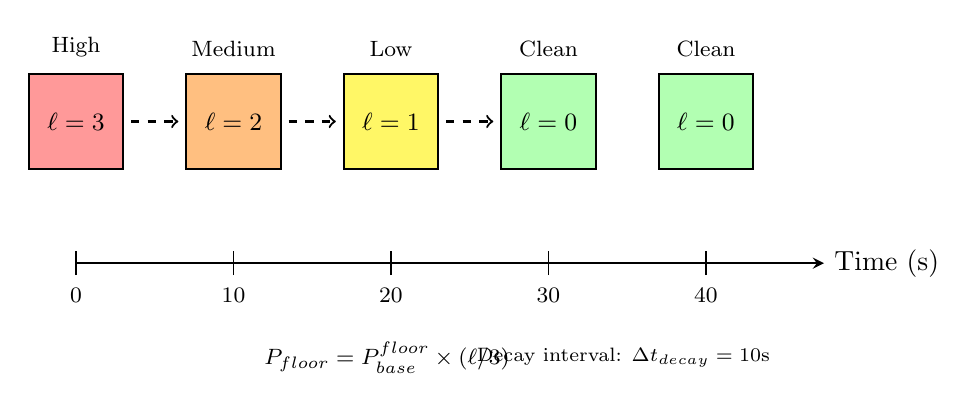
\begin{tikzpicture}[
    tile/.style={rectangle, draw, thick, minimum width=1.2cm, minimum height=1.2cm, font=\small},
    timeline/.style={->, thick, >=stealth},
    label/.style={font=\footnotesize}
]
    % Time axis
    \draw[timeline] (0,0) -- (9.5,0) node[right] {Time (s)};
    
    % Time markers
    \foreach \x/\t in {0/0, 2/10, 4/20, 6/30, 8/40} {
        \draw (\x, -0.15) -- (\x, 0.15);
        \node[below, label] at (\x, -0.2) {\t};
    }
    
    % Contamination level visualization at different times
    % t=0: Level 3 (red)
    \node[tile, fill=red!40] at (0, 1.8) {$\ell=3$};
    \node[above, label] at (0, 2.5) {High};
    
    % t=10s: Level 2 (orange)
    \node[tile, fill=orange!50] at (2, 1.8) {$\ell=2$};
    \node[above, label] at (2, 2.5) {Medium};
    
    % t=20s: Level 1 (yellow)
    \node[tile, fill=yellow!60] at (4, 1.8) {$\ell=1$};
    \node[above, label] at (4, 2.5) {Low};
    
    % t=30s: Level 0 (green)
    \node[tile, fill=green!30] at (6, 1.8) {$\ell=0$};
    \node[above, label] at (6, 2.5) {Clean};
    
    % t=40s: Still Level 0
    \node[tile, fill=green!30] at (8, 1.8) {$\ell=0$};
    \node[above, label] at (8, 2.5) {Clean};
    
    % Decay arrows
    \draw[->, thick, dashed] (0.7, 1.8) -- (1.3, 1.8);
    \draw[->, thick, dashed] (2.7, 1.8) -- (3.3, 1.8);
    \draw[->, thick, dashed] (4.7, 1.8) -- (5.3, 1.8);
    
    % Probability annotation
    \node[align=center, font=\footnotesize] at (4, -1.2) {
        $P_{\text{floor}} = P_{\text{base}}^{\text{floor}} \times (\ell/3)$
    };
    
    % Legend
    \node[align=left, font=\scriptsize] at (7, -1.2) {
        Decay interval: $\Delta t_{\text{decay}} = 10$s
    };
    
\end{tikzpicture}
\caption{Contamination decay timeline showing floor tile state transitions. A tile contaminated to level $\ell=3$ (red) decays by one level every $\Delta t_{\text{decay}}$ seconds (default: 10s), transitioning through medium ($\ell=2$, orange) and low ($\ell=1$, yellow) contamination levels before returning to clean ($\ell=0$, green). The floor transmission probability scales linearly with contamination level.}
\label{fig:contamination-decay}
\end{figure}

\subsubsection{Transmission Evaluation Algorithm}

Algorithm~\ref{alg:transmission-eval} presents the pseudocode for evaluating transmission events for a single HEALTHY agent, incorporating both proximity and floor contamination pathways.

\begin{algorithm}[t]
\caption{evaluateTransmission($a_i$, $\Delta t$)}
\label{alg:transmission-eval}
\begin{algorithmic}[1]
\REQUIRE Agent $a_i$ with $s_i = S$, frame delta $\Delta t$ (ms)
\STATE $P_{\text{scale}} \leftarrow \Delta t / 1000$
\FOR{each agent $a_j$ with $s_j = I$}
    \IF{$\|p_i - p_j\|_2 \leq r_{\text{inf}}$}
        \STATE $P_{\text{prox}} \leftarrow 1 - (1 - P_{\text{base}}^{\text{prox}})^{P_{\text{scale}}}$
        \IF{$\text{random}() < P_{\text{prox}}$}
            \RETURN \textbf{true} \COMMENT{Proximity transmission}
        \ENDIF
    \ENDIF
\ENDFOR
\FOR{each floor tile $f_k$ with $\ell_k > 0$}
    \IF{$a_i \in \text{AABB}(f_k)$}
        \STATE $P_{\text{floor}} \leftarrow P_{\text{base}}^{\text{floor}} \times (\ell_k / 3)$
        \STATE $P_{\text{floor}}^{\text{scaled}} \leftarrow 1 - (1 - P_{\text{floor}})^{P_{\text{scale}}}$
        \IF{$\text{random}() < P_{\text{floor}}^{\text{scaled}}$}
            \RETURN \textbf{true} \COMMENT{Floor transmission}
        \ENDIF
    \ENDIF
\ENDFOR
\RETURN \textbf{false} \COMMENT{No transmission}
\end{algorithmic}
\end{algorithm}

The algorithm prioritizes proximity transmission evaluation before floor contamination, reflecting the higher transmission risk of direct contact. The early-exit optimization on line 6 avoids unnecessary floor checks once proximity transmission succeeds. For a population of $n$ agents with $m$ contaminated tiles, the worst-case complexity is O($n + m$) per agent evaluation.

\subsubsection{Transmission Parameter Summary}

Table~\ref{tab:transmission-params} summarizes the key parameters governing transmission dynamics.

\begin{table}[t]
\centering
\caption{Transmission Mechanism Parameters}
\label{tab:transmission-params}
\begin{tabular}{@{}llcc@{}}
\toprule
Parameter & Description & Default & Unit \\
\midrule
$r_{\text{inf}}$ & Infection radius & 80 & pixels \\
$P_{\text{base}}^{\text{prox}}$ & Proximity transmission prob. & 0.3 & per second \\
$P_{\text{base}}^{\text{floor}}$ & Floor transmission prob. & 0.1 & per second \\
$\Delta t_{\text{decay}}$ & Contamination decay interval & 10000 & ms \\
$\ell_{\max}$ & Maximum contamination level & 3 & levels \\
\bottomrule
\end{tabular}
\end{table}

These parameters can be adjusted in the simulation configuration to model different contagion characteristics, such as more contagious variants (higher $P_{\text{base}}^{\text{prox}}$) or longer environmental persistence (higher $\Delta t_{\text{decay}}$).
